%% RedTwin: AI-Enabled Digital Twins for Continuous Red Teaming of
%% Open-Source Ecosystems
%%
%% NSF 26-506 (PESOSE), Track 3: Improving safety, security, and privacy.
%% Project Description.
%%
%% Compile with: pdflatex main.tex; bibtex main; pdflatex main.tex; pdflatex main.tex
%%
%% COMPLIANCE NOTES (NSF 26-506 + PAPPG 24-1):
%%   - Project Description limit for Track 3 is 15 pages, INCLUDING Results
%%     from Prior NSF Support. Check the page count after every edit.
%%   - NO URLs are permitted in the Project Description. Cite the open-source
%%     products via References Cited instead (PAPPG II.D.2.d(ii)).
%%   - Margins must be at least 1 inch on all sides, with no proposer-supplied
%%     information in the margins. No page numbers are printed, since
%%     Research.gov stamps its own.
%%   - Run `make check` (or see the note at the end of this file) to verify.

\documentclass[11pt,letterpaper]{article}

%% ---- NSF page geometry: 1-inch margins on all sides ----
%% No page numbers are printed: Research.gov stamps its own, and PAPPG II.C.2.c
%% forbids proposer-supplied information in the margins.
\usepackage[letterpaper,margin=1in,heightrounded,
            headheight=0pt,headsep=0pt,footskip=0pt]{geometry}

%% ---- Core packages ----
\usepackage[T1]{fontenc}
\usepackage[utf8]{inputenc}
\usepackage{times}
\usepackage{microtype}
\usepackage{setspace}

%% ---- Typography and layout ----
\usepackage{titlesec}
\usepackage{enumitem}
\usepackage{graphicx}
\usepackage{xcolor}
\usepackage{hyperref}
\usepackage{xurl}   % loads url; breaks long URLs so they stay inside the margin
\usepackage{booktabs}
\usepackage{longtable}
\usepackage{array}
\usepackage{xspace}

%% Single-spaced body text. PAPPG II.C.2.b allows up to six lines of text per
%% vertical inch; the value below yields ~5.7 lines/inch, inside that limit.
\singlespacing
\linespread{0.94}\selectfont
\setlength{\parindent}{1.5em}
\setlength{\parskip}{0.25ex plus 0.15ex}

%% Compact list spacing.
\setlist{topsep=0.3ex,itemsep=0.2ex,parsep=0pt,leftmargin=1.6em}

%% Keep long words and inline literals from intruding into the right margin.
\setlength{\emergencystretch}{2em}
\hbadness=10000

%% Tighter float separation (figure only; body font and margins unchanged).
\setlength{\textfloatsep}{8pt plus 2pt minus 2pt}
\setlength{\intextsep}{8pt plus 2pt minus 2pt}
\setlength{\abovecaptionskip}{4pt}
\setlength{\belowcaptionskip}{0pt}

%% ---- Section formatting (compact, NSF-style) ----
\titleformat{\section}
  {\normalfont\large\bfseries}{\thesection}{0.6em}{}
\titleformat{\subsection}
  {\normalfont\normalsize\bfseries}{\thesubsection}{0.5em}{}
\titleformat{\subsubsection}
  {\normalfont\normalsize\bfseries\itshape}{\thesubsubsection}{0.5em}{}

\titlespacing*{\section}{0pt}{0.9ex plus 0.2ex minus 0.2ex}{0.45ex plus 0.15ex}
\titlespacing*{\subsection}{0pt}{0.7ex plus 0.2ex minus 0.2ex}{0.3ex plus 0.15ex}
\titlespacing*{\subsubsection}{0pt}{0.7ex plus 0.2ex minus 0.2ex}{0.3ex plus 0.2ex}

%% Paragraph headings run in, with a little separation.
\titlespacing*{\paragraph}{0pt}{0.6ex plus 0.15ex}{0.5em}

%% ---- Hyperref settings ----
%% NOTE: the Project Description contains no URLs by design. urlcolor applies
%% only to the References Cited section.
\hypersetup{
  colorlinks=true,
  linkcolor=black,
  citecolor=black,
  urlcolor=blue!55!black,
  pdftitle={PESOSE: Track 3: RedTwin: AI-Enabled Digital Twins for Continuous
            Red Teaming of Open-Source Ecosystems},
  pdfauthor={Giovanni Vigna, Christopher Kruegel, Adam Doupe, Tiffany Bao}
}

%% ---- Convenience macros ----
\newcommand{\sysname}{RedTwin\xspace}

%% Conspicuous placeholder for information only the PIs can supply.
%% Set \todoverifyoff before submission to make any remaining ones fail loudly.
\newcommand{\todoverify}[1]{%
  \textbf{\textcolor{red}{[PI TO SUPPLY: #1]}}}

%% ---- No headers or footers ----
\pagestyle{empty}

\begin{document}

%% ===== Project Summary (1 page, separate upload in the NSF package) =====
%% ===== Project Summary (1 page) =====
%% NSF requires three labeled parts: Overview, Intellectual Merit, Broader Impacts.
%% The last line must carry 2-5 keywords (NSF 26-506, Section V.A).

\begin{center}
  {\large\bfseries Project Summary}\\[0.3em]
  {\large\bfseries PESOSE: Track 3: \sysname: AI-Enabled Digital Twins \\ 
  for Continuous Red Teaming of Open-Source Ecosystems}
\end{center}

\noindent\textbf{Overview}\\
Assessing the security posture of large computing infrastructures is
notoriously difficult. These are complex systems, dynamic in their
connectivity and usage patterns, and they often carry out processes that must
not be disrupted. Performing security analysis directly on a production
system can cause problems, as scans introduce overhead and analyzing services
for vulnerabilities can trigger crashes. Because of these risks, a security
assessment is usually performed manually, sporadically, and in an ad hoc
fashion by scarce human experts, while adversaries, now increasingly
augmented with AI, operate continuously. The goal of this proposal is the development of \sysname, an agentic framework
for the continuous, in-depth, and non-disruptive security assessment of
computing infrastructures built on open-source software. Such infrastructures
offer a unique opportunity for a new approach, because the openness of the
software enables the faithful replication of an infrastructure's topology and
service configuration. \sysname uses cooperating teams of AI agents to capture the configuration of
a target system, observe its execution, build a \emph{digital twin} of the
system, run red team exercises against the twin instead of the production
system, and, when vulnerabilities are found, guide a human-driven
verification and remediation of the issues in the original infrastructure.
Because the analysis runs on the twin, it can be repeated continuously and
adapted as the target evolves.

The ecosystem that this project targets is anchored on two existing, widely
deployed open-source products. The first is \textbf{nginx}, the reverse proxy
through which traffic enters and moves within nearly every open-source
deployment, and which we will harden against the memory-safety,
configuration, and request-smuggling defect classes that dominate its
history. The second is \textbf{ZMap}, the scanner with which operators
discover what is actually running, and which we will extend into an
instrument for safe, budgeted discovery inside production networks. Every
finding that we confirm on a twin is driven upstream to the project
responsible, and the work therefore improves not only individual deployments,
but also the shared ecosystem on which they are built.

\vspace{0.2ex}
\noindent\textbf{Intellectual Merit}\\
The \sysname framework contributes new agentic workflows that automate the
tedious tasks of capturing an infrastructure's configuration and reproducing
it in a virtualized environment. These workflows are supported by novel
techniques for replicating large-scale infrastructure at reduced scale while
preserving its security-relevant properties, and for measuring the
representativeness of the resulting twin through logic-based invariants and
attack-graph preservation analysis. A distinguishing feature of the approach
is that the fidelity of the twin is quantified rather than assumed, and that
the soundness of an analysis is reported together with a measure of how much
of the target system the capture process actually resolved. Vulnerability-analysis agents then examine the twin using novel techniques
for chaining vulnerabilities across a networked infrastructure, extending the
investigators' prior work on AI-planning-based privilege-escalation chains
and on a universal theory of in-program exploitation to complete
open-source ecosystems.

\vspace{0.2ex}
\noindent\textbf{Broader Impacts}\\
Open-source software underpins the Nation's critical infrastructure, from
health care and financial systems to utilities and government services. By
enabling continuous, non-disruptive security assessment of the ecosystems
built on this software, \sysname will improve the resiliency of that
infrastructure and help prevent attacks with catastrophic consequences. The improvements that the project contributes to nginx and ZMap
reach every downstream user of those products, including the many
organizations that cannot afford commercial alternatives. The project will
also produce open-source artifacts and a public corpus of reference
infrastructures, integrate infrastructure-security modules into the curricula
at UC Santa Barbara and Arizona State University, involve undergraduate students in research, and organize a new public capture-the-flag
competition centered on the creation of digital twins.

\vspace{0.2ex}
\noindent\textbf{Keywords:} critical infrastructure; open-source security; digital twins; AI agents; vulnerability analysis.

\clearpage

%% ===== Project Description (15-page limit) =====

\begin{center}
  {\large\bfseries Project Description}\\[0.3em]
  {\large\bfseries \sysname: AI-Enabled Digital Twins for Continuous\\
   Red Teaming of Open-Source Ecosystems}
\end{center}

%% --- Motivation and required Track 3 framing ---
\section{Introduction}
\label{sec:intro}

Assessing the security posture of large computing infrastructures is
notoriously difficult because they are complex systems, dynamic in their
connectivity and usage patterns, and they often carry out processes that
should not be disrupted. Performing security analysis directly on a
production system can cause problems: a single aggressive probe against a
database replica, a message broker, or an authentication service can cascade
into an outage that violates a regulated availability requirement, corrupts
state, or interrupts a process on which people depend.

Because of these risks, the analysis of the security posture of an
infrastructure is usually performed manually and in an ad hoc fashion, by
analysts whose expertise is scarce and expensive. As a result, these
assessments are carried out sporadically, and the evolution of the network
topology, the introduction of a new service, or a change in the configuration
of a component might introduce a vulnerability that invalidates the results
of the previous analysis. In the meantime, adversaries that are increasingly
augmented with AI operate continuously, automatically, and at
scale~\cite{measuring}. The proposed research targets this widening gap.

\textbf{The goal of the proposed research is to develop a new agentic
framework, called \sysname, to support the continuous assessment of the
security posture of computing infrastructures based on open-source
software.} \sysname uses cooperating teams of AI agents to capture the
configuration of a target system, monitor its execution, create a
\emph{digital twin} of the system, run red team exercises against the twin,
and guide a human-driven verification and remediation of the issues that are
found in the original system. The core principle of \sysname is a strict
separation between \emph{observation}, which is passive, non-disruptive, and
the only activity that ever touches the production system, and
\emph{analysis}, which is aggressive, potentially destructive, and confined
entirely to the digital twin. This approach is feasible because the components of the infrastructure are
open source, and therefore their behavior, configuration surface, and version
history are transparent and inspectable. This transparency makes it possible to run a
functionally equivalent instance of a component in a controlled environment,
something generally infeasible for closed, proprietary appliances.

\paragraph{A motivating scenario.}
Consider a regional health-care provider whose electronic health-record
system runs on a stack of open-source components: a
PostgreSQL~\cite{postgresql} cluster with streaming replication, a set of
application servers behind an nginx~\cite{nginx} reverse proxy, a
Keycloak~\cite{keycloak} identity provider federated with the hospital
directory, a RabbitMQ~\cite{rabbitmq} message broker connecting clinical
subsystems, and a fleet of medical-device gateways that speak proprietary
protocols. This deployment is subject to strict availability and privacy
requirements, and the security team cannot fuzz the application
servers, cannot flood the broker with malformed messages, and cannot run an
exploit against the identity provider. As a result, the questions that matter to the security team remain
unanswered. Can an attacker who compromises a
single device gateway pivot through the broker to reach patient records? Does
the proxy configuration expose an internal administrative endpoint through a
path that the access rules did not anticipate? Each of these questions concerns the \emph{deployment} as a whole, and none can be answered from an advisory or a source repository. \sysname is designed for this situation: it reconstructs the deployment as a
digital twin, exercises exactly these attack paths against the twin, and
reports the confirmed chains to the security team for verification on the
production system, all without ever sending a single aggressive packet to the
live infrastructure.

A possible alternative to a digital twin would be to leverage the staging
environment that engineers already use to test applications before
deployment. In practice, this would not be sufficient, as staging
environments are built and maintained manually, they drift from production as
the infrastructure evolves, and they are typically provisioned for functional
testing rather than to preserve the security-relevant structure of the
deployment: the exact component versions, the network reachability relations,
the trust and authentication dependencies, and the data that determines
authorization decisions. A staging environment that omits the device gateways, or that seeds an empty user directory, will not exhibit the attack paths exploitable in the real infrastructure. \sysname constructs a digital twin whose fidelity is measured and controlled
with respect to explicit security properties, as described in
Section~\ref{sec:thrust2}, and that is kept synchronized with the production
system by a continuous capture-and-observe loop, as described in
Section~\ref{sec:thrust1}.

\paragraph{Alignment with PESOSE Track~3 and contributions.}
This project is submitted to NSF~26-506, Track~3, which addresses
vulnerabilities in open-source products and infrastructure, including both
technical risks and socio-technical ones. The ecosystem we target is anchored on two existing, widely deployed open-source products, described in Section~\ref{sec:ecosystem}. The first is \textbf{nginx}~\cite{nginx,nginxsrc}, which we will harden against the memory-safety, configuration, and request-smuggling defect classes catalogued in Section~\ref{sec:landscape}. The second is \textbf{ZMap}~\cite{zmap,zmapsrc}, which we will extend into an instrument for safe, budgeted, and information-rich discovery inside production networks. Every finding that we confirm is driven upstream, so the work improves both
individual deployments and the shared ecosystem on which they are built.

The project contributes: (i) agentic workflows that capture the configuration
of an infrastructure into a continuously maintained knowledge base, together
with upstream extensions that make open-source discovery safe on production
networks; (ii) techniques for replicating large infrastructures at reduced
scale, supported by a \emph{quantitative fidelity measure}; (iii) methods for
chaining vulnerabilities across a networked infrastructure, extending our
prior work on AI-planning-based privilege escalation and on a universal
theory of in-program exploitation to the setting of complete ecosystems; and
(iv) the hardening of nginx and ZMap, a public corpus of reference
infrastructures with ground truth, and an open-source release of the
framework.

\section{The Target Open-Source Ecosystem}
\label{sec:ecosystem}

Track~3 asks proposers to improve the safety, security, and privacy of an
\emph{existing} open-source ecosystem. This project targets the ecosystem
that forms the observable and defensible perimeter of nearly every
open-source deployment, anchored on two widely used, publicly available
products: \textbf{nginx}~\cite{nginx,nginxsrc}, through which traffic enters
and moves within such deployments, and \textbf{ZMap}~\cite{zmap,zmapsrc},
with which operators discover what is actually running. \sysname hardens the
first, extends the second, and uses both as the concrete ecosystem against
which its methods are developed and evaluated.

\paragraph{nginx: the trust boundary of open-source infrastructure.}
nginx is an HTTP server, reverse proxy, load balancer, and TLS terminator
that has been released under the two-clause BSD license and that has been in
continuous development since 2004~\cite{nginx}. It ranks consistently among
the most widely deployed web servers in the world. The
\emph{development and testing model} follows a maintainer-review process
around a public repository~\cite{nginxsrc} and a development mailing list,
with periodic mainline and stable branches, an in-tree functional test suite,
continuous integration across a broad matrix of platforms and build
configurations, and downstream testing by the distributions that package it.
\emph{Dissemination} occurs through official binary packages, distribution
repositories, and container base images. The \emph{user base} spans
essentially every sector that runs open-source infrastructure, including the
health-care, financial, utility, and government deployments that this
proposal targets. The \emph{contributor base}, in contrast, is comparatively
small, and it consists of a core maintainer group, a set of occasional patch
contributors, and a large third-party module ecosystem that is maintained
outside the project. This asymmetry between an enormous user base and a concentrated maintainer base is precisely the structural risk PESOSE was created to address.

\paragraph{ZMap: discovering what is actually running.}
ZMap is a single-packet, stateless network scanner that has been released
under the Apache~2.0 license and that is maintained by an academic and
industrial consortium~\cite{zmap,zmapsrc}. Its stateless design allows a
single commodity machine to sweep enormous address spaces far faster than
connection-oriented scanners, and the companion ZGrab tool performs
application-layer handshakes that identify service software and
versions~\cite{zgrab}. The \emph{development and testing model} is a
pull-request-and-review process conducted in the open on GitHub, with unit
and integration tests that are run on every pull request and with tagged
releases that are packaged for major platforms. \emph{Dissemination} occurs
through the source repository, distribution packages, and container images,
and ZMap underpins commercial and non-profit internet-measurement services as
well as a substantial body of peer-reviewed research. The \emph{user base} includes network operators who perform asset inventory,
incident responders, attack-surface-management services, and academic
measurement groups, and the \emph{contributor base} is an active but modest
community centered on the maintaining institutions.

ZMap was designed for internet-wide measurement from outside a network, where
the marginal effect of a probe on any single host is negligible. This project
requires the opposite, that is, repeated discovery \emph{inside} a production
network whose hosts may be fragile medical, industrial, or embedded devices.
Applied naively, the very property that makes ZMap valuable, its speed, is what makes it unsafe here. Section~\ref{sec:thrust1} describes the extensions we will contribute upstream to make ZMap a first-class instrument for safe, budgeted, and information-rich discovery on production infrastructure.

\paragraph{The ecosystem view.}
These two products bracket the problem that \sysname addresses, as ZMap
determines what an operator can \emph{know} about an infrastructure without
disturbing it, and nginx determines what an attacker can \emph{reach} once
inside it. Both sit within a broader ecosystem that \sysname must also
capture, replicate, and analyze, including PostgreSQL~\cite{postgresql}, Keycloak~\cite{keycloak},
RabbitMQ~\cite{rabbitmq}, and Istio~\cite{istio}. Our working relationships with the maintainers and users of nginx and ZMap, documented in the accompanying letters of collaboration, give the project a direct path from a finding produced on a twin to a fix that reaches every downstream user.
        % required element (1) and (2)
\section{Societal, National, and Economic Impact}
\label{sec:impact}

nginx and ZMap sit beneath a large fraction of the open-source software
deployed today, and their defects are therefore inherited by every deployment
built on them.

\paragraph{What depends on nginx.}
nginx sits at the point where untrusted traffic first meets an
organization's software. It terminates TLS, enforces the first layer of
access control, routes requests to the application servers, and mediates
between the internet and the internal identity providers, brokers, and
databases. A defect or a misconfiguration at that point is rarely contained,
because it is a defect in the boundary that every other control assumes to be
intact. Hospitals, payment processors, utilities, and government services all
inherit this exposure, generally without any ability to audit it themselves.

\paragraph{What depends on ZMap.}
ZMap and the tools built on it are how defenders learn what they actually
operate. Attack-surface management, triage after a new advisory, incident
response, and regulatory asset inventory all reduce to the question of what
is running, where, and at what version. When that question is answered incompletely, every downstream decision
inherits the gap, because hosts absent from the inventory are not patched when
an advisory lands. Improving the safety and the
information yield of open-source discovery therefore improves the security of
every organization that relies on it, and it disproportionately helps those
that cannot afford commercial alternatives.

\paragraph{Economic and national significance.}
These components are deployed across the sectors on which the Nation depends,
and the open-source stack as a whole has recently been valued in the
trillions of dollars annually. The maintainer asymmetry described in
Section~\ref{sec:ecosystem} means that public investment in the security of
these specific components generates returns far out of proportion to its cost:
every vulnerability that \sysname finds and drives upstream is removed
simultaneously from every deployment that shares the affected component.

\paragraph{Measures of success.}
The project advances several of the measures of success named in the
solicitation. It establishes new \emph{data sets}, in the reference
infrastructures, their ground-truth knowledge graphs, and the seeded
vulnerability corpus of Section~\ref{sec:evaluation}; \emph{new technologies
and techniques}, in the capture, replication, fidelity-measurement, and
exploitation-chaining methods of Thrusts~1--3, all released as open source;
and new \emph{research infrastructure}, in the twin-construction toolchain
and the public twinCTF infrastructure. Finally, it prepares participants for
careers in \emph{STEM} through the activities of
Section~\ref{sec:broader}.
                  % Track 3: societal/national impact
\section{Targeted Vulnerabilities and Risks}
\label{sec:landscape}

\paragraph{Memory-safety defects in C network services.}
nginx is written in C, and it parses attacker-controlled input at the network
edge. Its history contains exactly the defects that this implies. Examples
are a stack buffer overflow that is reachable through chunked transfer
encoding~\cite{cve2013:nginx}, an off-by-one heap write in the DNS resolver
that was remotely triggerable across a twelve-year span of
versions~\cite{cve2021:resolver}, and repeated memory-disclosure defects in
optional modules that many operators did not know they had compiled
in~\cite{cve2022:mp4}. These are the defects that the component-level analysis of Section~\ref{sec:thrust3} targets, and they are why that analysis cannot be run against production.

\paragraph{Configuration-induced vulnerabilities.}
The larger practical risk is not a flaw in nginx, but a flaw in the way that
nginx was configured. The directive language admits well-documented footguns
whose consequences are severe and whose presence is invisible to the
operator. For example, an \texttt{alias} directive without a trailing slash
yields path traversal, disabling slash merging in front of an upstream that
normalizes differently yields an access-control bypass, a
\texttt{proxy\_pass} directive that uses a variable silently disables URI
normalization, and parsing mismatches between nginx and its upstream enable
request smuggling~\cite{cve2019:smuggling}. This class of defect is systemic
rather than incidental, and it has been shown to generalize across proxies
and application servers~\cite{orangetsai}. Crucially, these vulnerabilities exist only in the \emph{deployed configuration}, and cannot be found by
analyzing the nginx source alone, nor in a staging environment that does not reproduce production. They are the paradigmatic case for a fidelity-controlled twin.

\paragraph{Cross-component chains.}
The findings that matter most are compositions: a permissive proxy rule that
exposes an internal endpoint, combined with a deserialization flaw in a
client library, combined with a credential that is reachable from the
compromised service. Each link in such a chain may be individually
unremarkable, but the chain as a whole is critical.

\paragraph{Socio-technical risks.}
Deployments do not install nginx. They install a container image, a distribution package, or an ingress
controller, such as \texttt{ingress-nginx}, that contains some build of nginx, with some set of modules, at some version, and from some registry. The
Log4Shell incident showed how a defect in a transitive dependency propagates
instantly across every system that unknowingly embeds it~\cite{log4shell}.
\sysname records provenance and Software Bills of Materials in the knowledge
base, as described in Section~\ref{sec:thrust1}, so that the analysis can
reason about attack paths that originate in a dependency which the operator
never chose explicitly. In doing so, we follow the recommended practices of
CISA and NSA~\cite{cisansa} and the criteria of the OpenSSF~\cite{openssf}.
Two further risks are in scope. First, the \emph{third-party module}
ecosystem of nginx is maintained outside the core project and receives a
fraction of its scrutiny, yet modules are compiled into the same address
space with the same privileges, and an unmaintained module is thus an
unpatched vulnerability that has no advisory to trigger an update. Second,
the concentration of \emph{maintainer and governance} authority is itself a
security property, as the xz-utils backdoor showed that a patient adversary
can obtain maintainer trust and introduce a backdoor that survives ordinary
review~\cite{xzbackdoor}.
%And \emph{insider and
%poisoned-component} risk is covered because the Red Team Agents plan from
%arbitrary initial footholds, so an adversary holding valid credentials or
%controlling a build artifact is expressible as a starting condition in the
%same planning formulation.

\paragraph{Prior incidents and threat model.}
These classes of defect are not hypothetical, and the incidents that
instantiate them share a structure that motivates the design of this project.
The clearest example is the set of defects that were disclosed in 2025 in the
\texttt{ingress-nginx} admission controller, collectively named
``IngressNightmare,'' which permitted unauthenticated remote code execution
and the disclosure of cluster-wide secrets on a large fraction of Kubernetes
deployments~\cite{ingressnightmare}. The relevant point is not the defect itself, but its reachability, as whether a given cluster was exploitable depended on the network policy, on whether the controller was reachable from the workload pods, and on the surrounding configuration. That question is answerable only against a faithful replica, and it is exactly the question no operator could safely ask of production. The same structure recurs in the resolver defect of 2021, whose
exploitability depended on whether an attacker could influence DNS responses
from the network position of the deployment~\cite{cve2021:resolver}, and in
request smuggling, which depends on the specific pairing of proxy and
upstream~\cite{cve2019:smuggling,orangetsai}. In every case, the advisory
establishes that a defect exists, and only the deployment determines whether
it matters.

Accordingly, we consider an adversary whose goal is unauthorized access to a
designated high-value asset, such as a patient database, a credential store,
or a cluster control plane. We model four initial positions: an
\emph{external} adversary, who has network access only to internet-facing
services; a \emph{foothold} adversary, who has compromised one low-privilege
component; an \emph{insider} adversary, who holds valid credentials for one
role; and a \emph{supply-chain} adversary, who controls one dependency or
build artifact. The adversary is assumed to know the open-source composition
of the infrastructure, since that information is public, but not its
deployment-specific configuration or its secrets. Two assumptions bound the
work. First, \sysname evaluates the security of the \emph{deployment}, and physical
attacks, social engineering, and the compromise of the virtualization
platform are out of scope. Second, \sysname never attacks the production
system, and any conclusion about production is therefore bounded by the
measured fidelity of the twin, which Section~\ref{sec:thrust2} makes
explicit and quantitative rather than assumed.
 % Track 3: vulnerabilities + risks

%% --- Development plan ---
\section{Technical Approach and Research Thrusts}
\label{sec:approach}
\label{sec:thrusts}

\sysname creates a digital twin of an infrastructure, performs security tests
on the twin, and uses the results to improve the security posture of the
original. Three challenges shape the design. First, the configuration of the
original must be captured continuously, as complex infrastructures are in
constant evolution. Second, most large infrastructures cannot be fully
replicated, and the twin must be smaller in scale but still representative. Third, as the infrastructure evolves, the twin has to evolve
as well, or the results will describe a system that no longer exists.

\begin{figure}[!htbp]
\centering
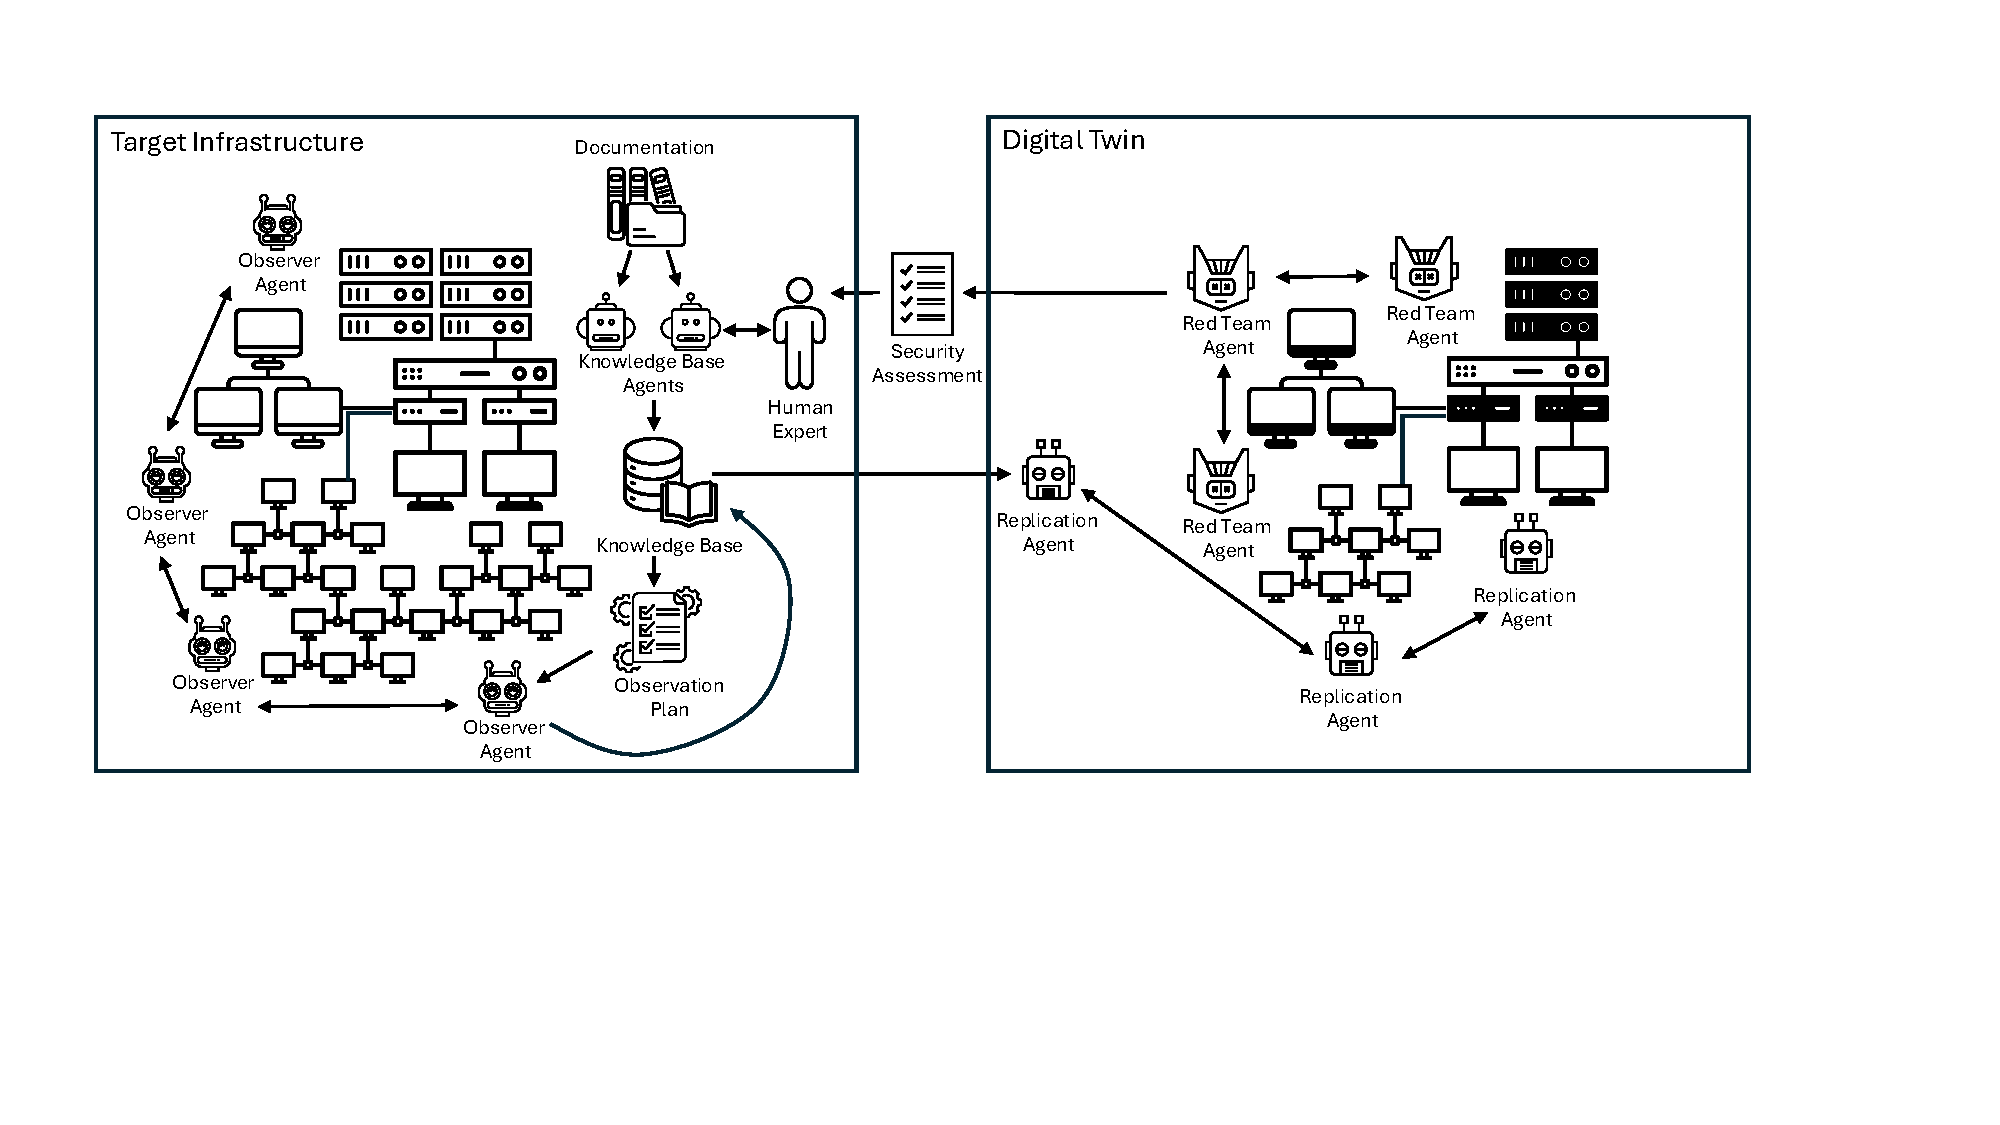
\includegraphics[width=\linewidth]{figures/redtwin_architecture.pdf}
\caption{Overview of the \sysname framework. Knowledge Base Agents combine
documentation with human expertise to build a Knowledge Base, driving an
Observation Plan that deploys Observer Agents, which collect dynamic
information without disrupting operations and feed it back. Replication
Agents construct a digital twin from the Knowledge Base, and Red Team Agents
continuously assess that twin, producing findings that are verified and
remediated on the target infrastructure.}
\label{fig:overview}
\end{figure}

\sysname addresses these challenges by leveraging four cooperating teams of
agents, summarized in Figure~\ref{fig:overview} and developed in the thrusts
below. The Knowledge Base Agents build and maintain the model of the target,
the Observer Agents enrich that model by watching the running system without
ever touching it, the Replication Agents construct the twin, and the Red Team
Agents attack the twin and report their findings to a human analyst. When a
finding is a false positive, or an artifact of an imprecise replication, the information flows back to the Knowledge Base and Observer Agents, so each
analysis cycle also improves the fidelity of the twin. In the health-care deployment of
Section~\ref{sec:intro}, this loop is what turns an undocumented
administrative endpoint, a permissive \texttt{proxy\_pass} rule, and a
deserialization flaw in a broker client library into a single reported chain
from a device gateway to the patient database.

\subsection{Thrust 1: Capturing Open-Source Infrastructure Configurations}
\label{sec:thrust1}

\paragraph{Knowledge base design.}
Structured data will be used to represent the network topology and the roles
of the various components. For this layer, we will use a graph database, such
as Neo4j~\cite{neo4j}, whose model is a natural fit for the questions that
\sysname must answer, such as which hosts can reach a given service, which
services share a credential store, and which paths connect an externally
exposed component to a sensitive asset, while a vector store, such as
Qdrant~\cite{qdrant} or Weaviate~\cite{weaviate}, will hold the
natural-language documentation. A research challenge in this
step is the design of a schema expressive enough to capture the
security-relevant structure of an arbitrary deployment, yet constrained
enough to support the queries and invariants used downstream. We will model
hosts, containers, services, network segments, credentials, data stores, and
trust relationships as typed nodes and edges, and we will attach to each of
them the \emph{provenance} of the information together with a
\emph{confidence} level. Both are essential, because the same fact may be
asserted by a configuration manual and contradicted by a runtime observation.
Version information must be fine enough to map a deployed component to the
package, release, and build options that determine its vulnerabilities, since the component name alone does not identify a vulnerability set, whereas
the version, the module set, and the directive configuration do.

\paragraph{Observation techniques.}
The Observer Agents monitor the system statically, through documentation,
code, configuration files, and infrastructure-as-code artifacts, and
dynamically, through the runtime observation of network and host activities.
Examples of these techniques are passive network analysis at key north-south
and east-west points, the interpretation of logs into a shared ontology by
means of LLMs, API monitoring through facilities such as eBPF or service
meshes like Istio~\cite{istio}, configuration monitoring through managers
such as Ansible~\cite{ansible} or Puppet~\cite{puppet}, and the ingestion of
alerts from IDS/IPS, EDR, or SIEM tools. In addition, we plan to extend our
previous work on service security dependency analysis~\cite{achilles}. That
research demonstrated that by observing the dynamic behavior of services it
is possible to derive their security properties and dependencies. Accurately modeling these dependencies is essential: any dependency missed
during capture is absent from the twin and therefore never exercised by the
analysis.

\paragraph{Safe active discovery: extending ZMap.}
Passive observation cannot resolve every question, because whether a service
is reachable from a given segment, and what version it runs, is often
answerable only by sending a packet. The stateless design of ZMap~\cite{zmap} makes it
the right foundation for this task, but its assumption that the marginal
effect of a probe is negligible does not hold inside a hospital or a plant.
We therefore plan to develop, and contribute upstream, four extensions:
\emph{impact-budgeted scheduling}, that imposes per-target budgets on probe
rate and concurrency derived from what the knowledge base records each host
to be, with hard interlocks that abort a sweep when the observed latency or
error rates degrade; \emph{knowledge-graph-native output}, that emits typed assertions with provenance and confidence, so discovery feeds
the schema directly; \emph{richer safe fingerprinting}, that extends the
ZGrab~\cite{zgrab} handshakes to recover the version and module detail needed
to map a service to an upstream package; and \emph{incremental re-scan},
that prioritizes re-probing where confidence has decayed. These extensions
address the reason why many operators decline to scan their own networks, and
they are a concrete Track~3 improvement to a widely used product.

\paragraph{Observation planning and coverage.}
We will formulate the synthesis of the observation plan as a constrained
optimization problem. Each candidate vantage point offers a certain amount of
information gain, at a cost expressed in terms of the load on the production
system, the intrusiveness of the deployment, and the consumption of scarce
resources such as LLM queries, and the plan maximizes the coverage of the
components most relevant to the security model while respecting hard
constraints, for example, never deploying an agent on a host that carries a
latency-sensitive clinical workload. Because observation is deliberately
non-aggressive, the resulting model is necessarily incomplete. We will therefore develop a
\emph{model coverage} metric that estimates what fraction of the infrastructure the capture has
resolved, using saturation analysis over observation time, cross-validation
among documentation, infrastructure-as-code, and runtime observation, and, on
the reference networks, direct measurement against withheld ground truth.
Coverage is reported alongside every finding, and it bounds every claim
\sysname makes about production.

\paragraph{Supply chain and the human loop.}
In addition, we will incorporate SBOMs and package manifests into the capture process, so the
knowledge base records not just what is running, but also where each
component came from. This addresses the socio-technical risks
described in Section~\ref{sec:landscape}, and it feeds the remediation loop
of Thrust~3. Note that, while the process is presented here as a sequence,
the agents will actually work continuously: new documentation triggers new
observation plans, and observations inconsistent with the documentation are
presented to the administrator for disambiguation. We envision this
as an agent-human collaboration, because deploying observer agents modifies
the infrastructure and must be vetted, but as the agents become more
knowledgeable, we expect that the level of interaction will diminish, and
Section~\ref{sec:evaluation} measures whether it does.

\subsection{Thrust 2: Replicating Computing Infrastructures}
\label{sec:thrust2}

The key problem in this thrust is how to build digital twins that are
scale-reduced and yet still representative of the original. We organize the
approach around three insights, and we then make faithfulness quantitative.

\paragraph{Insight 1: infrastructures replicate for load.}
If 200 file servers share the same operating-system image, package versions,
and firewall rules, they can be considered equivalent from a security
modeling perspective, and a single instance can stand for all of them. This reduces the veracity of the twin, because attacks that exploit resource
bottlenecks will not transfer. The abstraction is therefore a trade-off
between faithful replication and the minimization of resource usage, and the
fidelity measure defined below reports where a given twin sits on it. We will formalize this idea as an equivalence relation over the
components of the infrastructure. Two components are placed in the same class
when they agree on the attributes that determine their security behavior,
such as the software image and version, the set of open ports and exposed
services, the applicable firewall and access rules, the trust relationships
in which they participate, and their position in the network topology. The
twin then instantiates a single representative per class, together with a
\emph{multiplicity annotation}. A central research question is which
attributes must be included to preserve a given class of attacks, and we will
study it empirically, by measuring whether the attacks discovered on the
abstracted twin still succeed when the abstraction is refined, and
analytically, by relating the attributes to the preconditions of the attack
primitives modeled in Thrust~3. Clustered services are the hard case, since
collapsing replicas erases node membership, quorum, and inter-node trust; a
RabbitMQ~\cite{rabbitmq} cluster, with input from its maintainers, is our
stress test for the relation.

\paragraph{Insight 2: services operate in patterns.}
Network administrators tend to reuse combinations of components that work
well and with which they are familiar, and a particular pairing of a proxy
and an upstream recurs throughout an infrastructure. Each pattern can
carry pattern-specific vulnerabilities, and the replication algorithm will
identify these patterns and will make sure that each of them is instantiated
in the twin. This matters directly for our anchor product: request smuggling is a property
of a \emph{pairing} and not of nginx alone, so a twin that collapses distinct
pairings into one cannot exhibit those defects.

\paragraph{Insight 3: data is as relevant as code.}
If an LDAP server uses a specific database of users to authorize access to a
host, that data determines whether an attack path exists. Organizations
usually have to deal with three types of data. \emph{Semantic data}
represents the things the organization deals with, such as patients,
diagnoses, and insurance claims. \emph{Structural data} defines the shape of
the production data systems, including schemas, foreign-key relationships,
record counts and sizes, and, in the case of hospitals and other health-focused organizations, domain objects such as DICOM images or FHIR
resources. \emph{Operational data} reproduces how the infrastructure behaves,
including login frequency, API request patterns, query mixes, and backup
jobs. Specialized agents will profile the source environment for the
aggregate properties required for fidelity, will generate a semantically
consistent synthetic state, and will enforce invariants such as referential
integrity, protocol semantics, and causal ordering.
In the context of health-management infrastructures, such as hospitals, we plan to leverage existing open-source medical datasets to create realistic datasets.
To this end, we include a letter of support from the CEO of Sage Bionetworks, an organization whose goal is to provide access to open-source medical and health-related datasets. 
Using the datasets managed by Sage Bionetworks as well as those that are brokered by that organization, we are planning to create high-fidelity synthetic datasets that will maintain the characteristics of real-world medical data.

\paragraph{Reconciling sanitization with authorization.}
Sanitization and the preservation of security behavior are in direct tension,
because authorization outcomes frequently determine whether an attack path
exists. For example, replacing real users with synthetic ones can silently
remove the group membership that made a privilege escalation possible. We
will therefore specify the \emph{authorization structure} separately from the
\emph{data content}. Identities, groups, roles, ACL entries, and the
membership and delegation edges among them will be reproduced as an
isomorphic graph that preserves the cardinalities and the shape of every
permission relation, while the identifying content is replaced. Secrets
become surrogates of equivalent strength and \emph{distribution}, preserving
the properties an attacker could exploit, such as the reuse of one credential
across services. Determining which authorization-relevant
properties must be preserved exactly, which only distributionally, and which
can be discarded is a research question of this thrust.

\paragraph{Making fidelity quantitative.}
Once the twin has been created and the data instantiated, we must analyze its
configuration with respect to the original infrastructure, and to this end we
will extend graph- and metric-based comparison algorithms~\cite{comparing}.
We plan to approach this problem in two ways. First, we will develop
techniques to represent the properties of the network using logic-based
approaches. These properties could define access, for example, ``service X is
reachable from host Y'', or topology, for example, ``the cluster Z can only
be accessed through host W'', and they are then treated as invariants that
must be preserved by the replication process. Determining what properties are
important to represent the security posture of a network, and how they can be
verified, is an integral part of the research, and it connects to work on
network configuration verification~\cite{batfish,minesweeper}.
Second, we will perform an attack-graph preservation analysis. We will
generate attack graphs~\cite{attackgraphs,mulval} for both the original
infrastructure and the twin, and we will establish that the attack graphs of
the twin are a sound abstraction of the attack graphs of the original.
Building on these two techniques, we will define a fidelity measure that
reports which security-relevant properties are preserved, which are
approximated, and which are lost. The measure rests on two distinct notions.
\emph{Soundness} is the property that every attack path present in the
original has a corresponding path in the twin. It is what the
equivalence-class abstraction is constructed to preserve, and it either holds
or it fails; the quantity we can measure against ground truth is
\emph{attack-path recall}, the fraction of the original's attack paths that a
given twin reproduces. Recall below one therefore identifies a defect to be
diagnosed and not a tolerance to be accepted: some abstraction decision
discarded an attribute on which an attack depended, and the missing path
identifies which one. \emph{Precision} is the fraction of the paths in the
twin that correspond to real paths in the original, and the abstraction trades
precision away deliberately, so a Thrust~3 finding that does not reproduce
likewise localizes to a specific abstraction decision that the Replication
Agents can then refine. 

%Finally,
%because the search over the action space of the planner dominates the cost of
%Thrust~3, we will also investigate a learned prioritization over the discrete
%planning action space, and Section~\ref{sec:evaluation} ablates it, as the
%planner functions on knowledge-base heuristics alone.

\paragraph{What soundness can and cannot mean here.}
Soundness, as defined above, carries a specific limit. The attack
graph of the original can only be derived from the captured model, itself the
product of deliberately non-aggressive observation. What we can establish is therefore \emph{soundness relative to the captured
model}, and not an unconditional claim about the physical system. On the reference
networks, where ground truth exists by construction, we will evaluate the
stronger property, by comparing the attack graph of the twin against one
derived from the true configuration, and on production every soundness claim
is reported jointly with the model coverage metric of Thrust~1.

\paragraph{Components that cannot be replicated.}
For proprietary appliances, unavailable hardware, and closed-source services
for which no substitute exists, the Replication Agents will synthesize a mock
that reproduces the externally observable behavior recorded by the Observer
Agents. Mocks introduce \emph{false negatives} by construction: a mock reproduces only
the behavior the Observer Agents recorded, and exploitable behavior is
frequently behavior that was never exercised in production. We therefore treat every mocked
component as a declared region of unsoundness. The fidelity report marks
which parts of the attack surface are mock-backed, findings whose chains
traverse a mock are flagged as requiring verification on the production
system, and the coverage measure is reduced accordingly. Our previous
research on re-hosting proprietary
firmware~\cite{gustafson2019:pretender,gustafson2020:halucinator,spensky2021:Conware,scharnowski22:fuzzware}
provides the starting point: it demonstrated that static and dynamic analysis
combined with runtime observation can execute proprietary firmware on emulators
such as Qemu~\cite{qemu}, even without documentation about the underlying
hardware.

\subsection{Thrust 3: Analyzing the Security Posture of Digital Twins}
\label{sec:thrust3}

This thrust combines component-level techniques, such as
fuzzing~\cite{fleischer23:actor,scharnowski22:fuzzware}, static
analysis~\cite{machiry17:drchecker}, and symbolic
execution~\cite{ruaro21:syml}, with system-level attacks, such as multi-step
breaches~\cite{redini20:karonte}. Our previous work in the DARPA AIxCC
competition, in which we developed the Artiphishell
system~\cite{artiphishell}, has shown that the problem of identifying
complex, multi-step vulnerabilities can be formulated effectively using
agentic workflows. The Red Team Agents orchestrate these established
techniques rather than reinventing them, selecting and configuring the
appropriate tool for a given service and interpreting the results in the
context of the knowledge base. The value added by the agentic layer is
twofold: it maps a low-level defect to the role that the affected component
plays in the infrastructure, and it expresses the defect as an exploitation
primitive with preconditions and postconditions that the system-level planner
can compose. Here the open-source nature of the ecosystem is an advantage: the source and
the build configuration of each component are available, and the agents can
analyze them with a depth that would be impossible for closed appliances.

\paragraph{Hardening nginx.}
nginx is the first target of this machinery, and it is the primary vehicle
through which this project delivers Track~3 outcomes upstream. We will pursue
this along three lines. For \emph{memory safety}, we will apply our fuzzing
and static-analysis tooling~\cite{fleischer23:actor,machiry17:drchecker} to
the request and response paths and to the optional modules that historically
carry defects, running against twin-hosted instances configured exactly as
they are configured in the deployments we capture, reaching configurations
that the upstream test suites do not exercise. For
\emph{configuration-induced vulnerabilities}, we will use the record of real
deployed directive configurations held in the knowledge base to build a
checker that identifies the traversal, normalization, and access-bypass
patterns of Section~\ref{sec:landscape}, and we will contribute the resulting
rules as tooling that the wider community can run. For \emph{request
smuggling}, we will exercise the proxy-upstream \emph{pairings} as they
actually occur in captured deployments, differentially testing how nginx and each upstream parse the same request.
Such defects are properties of the pair, and testing either component in
isolation cannot reveal them. Confirmed defects are reported upstream
under the process of Section~\ref{sec:buildtest}. Where a defect is configuration-induced instead of a code flaw, the
deliverable is detection tooling and documentation, since there is no patch to
submit.

\paragraph{Composing multi-step attacks.}
The workflow will instantiate a clean version of the twin, and the attack
planning will have access to the knowledge base, so that the planner reasons
with the information available to the knowledgeable adversary of
Section~\ref{sec:landscape}. The combination of single attacks will build on
top of the model of preconditions and postconditions of attacks that we have
explored in our ChainReactor~\cite{chainreactor} and UTE~\cite{ute} research
efforts. ChainReactor automated the discovery of privilege-escalation chains
via AI planning. UTE, which we have developed as part of the DARPA HARDEN
program, treats exploitation as a search problem: any exploitable bug exposes
a small set of operations that an attacker can induce, for example
allocations, frees, reads, writes, and file operations, and by modeling the effects and the preconditions of these operations
abstractly, the construction of an exploit becomes tractable for a solver. Furthermore, this same
abstraction allows us to reason about chains that cross theories, for
example, a buffer overflow that exists only if the attacker can control the
contents of a file. UTE has been designed for
in-program analysis and ChainReactor for in-host analysis, and
\textbf{extending and combining both of them to reason across a networked
infrastructure is a core research contribution of this thrust.} The planning
activity targets a designated high-value asset, and unauthorized access to
that asset demonstrates a breach. To scale to infrastructures with many
hosts, we will exploit the same equivalence-class structure used for
replication, as an attack step feasible against one representative of a class
is feasible against every member. This lets the planner reason at the level
of classes and roles rather than individual hosts, and then lift a discovered
chain into a family of concrete chains in the original.

\paragraph{What ``continuous'' costs.}
\sysname operates on three cadences:
\emph{event-triggered} re-capture, within minutes of an
infrastructure-as-code commit or of an observer detecting an undocumented
host; \emph{scheduled} re-analysis, nightly for the component-level analysis
of changed components and weekly for the full multi-step planning; and
\emph{advisory-triggered} re-analysis, when a new CVE affects a component
that the knowledge base records as deployed, reducing the question of whether
the organization is exposed from a multi-day manual exercise to a
query against a twin that already exists. The dominant recurring costs are LLM inference and the compute for twin
instantiation and fuzzing. Establishing the cost per cycle, and reducing it
through incremental re-capture and caching, is an explicit engineering
objective, and Section~\ref{sec:evaluation} reports it as a metric.

\paragraph{From findings to prevention, detection, and recovery.}
Consistent with the goals of PESOSE Track~3, the output of this thrust is oriented toward prevention, detection, and
recovery. The result of an analysis is a detailed document that describes the
multi-step attack, and this document is communicated to a human security
analyst, who will have to validate the findings on the actual system. False positives trigger a re-evaluation of the fidelity of the replication, so
this thrust both produces actionable findings and improves the twin. Each confirmed chain is accompanied by the
set of preconditions that enabled it, which directly suggests remediations,
such as removing an unnecessary reachability relation, updating a component
to a patched release, tightening an access-control rule, or segmenting a
trust boundary. When a finding traces to a defect in an upstream component,
the provenance captured in Thrust~1 identifies the project responsible, and
the chain serves as a high-quality report. Furthermore, because \sysname
produces attack graphs, the same artifacts can be used to prioritize
monitoring and to inform recovery planning, by identifying the choke points
whose compromise would be most damaging.

\section{Build and Test Infrastructure, Quality Control, and Disclosure}
\label{sec:buildtest}

\paragraph{Build and test infrastructure.}
\sysname is developed in a public monorepo, and every change is submitted as a
pull request that must pass continuous integration before it is reviewed. The
suite includes unit tests for the tooling of each agent team, integration
tests that exercise capture, replication, and analysis end to end against a
small reference infrastructure, and regression tests derived from every
previously confirmed finding, so that a capability once demonstrated cannot
be silently lost. Because the outputs are produced by non-deterministic
agents, the integration suite executes each scenario multiple times and
asserts on \emph{distributions} of outcomes rather than on exact traces, and
the run-to-run stability is tracked as a reported metric. The reference
infrastructures are themselves infrastructure-as-code, versioned alongside the source, so any result can be reproduced from a
commit hash.

\paragraph{Quality control and security of new content.}
Contributions require the review of a project maintainer, and they must pass
automated checks before they are merged, including static analysis and
linting, dependency scanning against advisory databases, and a verification
that any new dependency is recorded in the SBOM of the project. Releases are
tagged, signed, and published together with a generated SBOM and a provenance
attestation, following the recommended practices of CISA and NSA~\cite{cisansa}
and targeting the best-practices criteria of the OpenSSF~\cite{openssf} and
the build-provenance levels of SLSA~\cite{slsa}. Content generated by agents receives specific scrutiny. For example, twin
configurations, mocks, and synthetic datasets each carry a manifest that
records what produced them and with what confidence, and the synthetic data
is validated by the constraint agents of Section~\ref{sec:thrust2} and
checked to contain no material derived from production records. Twins are
held in isolated networks, access to them is restricted to the project team
and to the owning organization, and they are destroyed at the end of an
engagement.

\paragraph{Licensing and upstream contribution.}
\sysname will be released under a permissive OSI-approved license matching
those of the anchor products (BSD-2-Clause for nginx, Apache~2.0 for ZMap),
so contributions can flow upstream without license friction, and the reference infrastructures and their ground-truth knowledge
graphs will be released under a permissive data license. Improvements to the
anchor products are developed as upstream contributions from the start,
following the process of each project rather than being maintained as a fork.
For example, the ZMap extensions will be submitted as pull requests with
tests~\cite{zmapsrc}, and the nginx findings will follow the nginx security
process. Where a finding concerns a deployment configuration rather than
component code, the deliverable is detection tooling and documentation
contributed to the community.

\paragraph{Responsible disclosure and dual use.}
\sysname automates the discovery of exploitable chains in widely deployed
open-source software, and we treat the resulting dual-use considerations
explicitly. All findings follow coordinated vulnerability disclosure, in that a confirmed
upstream defect is reported privately to the security contact of that
project, together with a reproducer and a proposed remediation, and
publication is withheld until a fix is available or until a standard embargo
period has elapsed. Findings specific to the deployment of a partner belong
to that partner. The assessment of any system is performed only under a written authorization
from its owner, specifying the scope, the permitted observation techniques,
and the rules of engagement. The campus evaluations of Section~\ref{sec:evaluation} are conducted under
agreement with the responsible IT organizations at UCSB and ASU, with the
impact interlocks of Section~\ref{sec:thrust1} enforced throughout, and we
will seek IRB review where any activity touches human-subjects data. We will
publish the framework, the reference infrastructures, and the methods in
full, because defenders cannot use what they cannot obtain, and because the
capability we automate is one that sophisticated adversaries already
possess~\cite{measuring}. However, we will not publish weaponized exploits
for unpatched defects, and the released artifacts require an authorization
scope before an assessment can be run.
              % Track 3 review criterion 4

%% --- Assessment ---
\section{Evaluation Plan}
\label{sec:evaluation}

\paragraph{Reference infrastructures.}
Evaluating capture and replication requires ground truth that production systems rarely provide, and we will construct a
suite of reference networks for which the topology, the configuration, and the set of planted
vulnerabilities are fully known to us. These networks will be built from
widely deployed open-source components, including our anchor products and the
databases, brokers, identity providers, and orchestrators that surround them,
and they will be described entirely through infrastructure-as-code, so we can instantiate
them reproducibly, vary their scale, and generate the
ground-truth knowledge graph automatically. We have developed substantial
expertise in this domain through our work on the Global Accessible Test
Infrastructure (GATE) as part of the ACTION NSF AI
Institute~\cite{action}, in which we have created topologies that represent
smart cities, chemical plants, water systems, and manufacturing plants. We
will seed each reference network with a mixture of known vulnerabilities that
are drawn from public advisories, including the nginx defect classes of
Section~\ref{sec:landscape}, and with deliberately introduced
misconfigurations. In addition, we will design a subset of the networks to
require genuine multi-step chains, so success cannot be achieved by finding a
single isolated flaw. These reference networks will also serve as
the challenges for the twinCTF competition described in
Section~\ref{sec:broader}, and they will be released as a public benchmark.

\paragraph{Metrics and targets.}
Targets are stated for the reference networks, where ground truth exists.

{\footnotesize\setlength{\tabcolsep}{4pt}\renewcommand{\arraystretch}{0.93}
\begin{longtable}{@{}p{0.55\linewidth}p{0.42\linewidth}@{}}
\toprule
\textbf{Metric} & \textbf{Target}\\
\midrule
\multicolumn{2}{@{}l}{\emph{Thrust 1 --- capture}}\\
Hosts and services correctly identified & $\geq 95\%$ of ground truth\\
Service dependencies correctly identified & $\geq 90\%$\\
Model coverage estimate vs.\ measured & within 10 points\\
Expert input per 100 hosts & $\leq 4$ h, declining across cycles\\
Production impact during observation & no measurable latency or error change\\
\addlinespace[2pt]
\multicolumn{2}{@{}l}{\emph{Thrust 2 --- replication}}\\
Attack-path recall (paths preserved) & $\geq 90\%$\\
Precision (twin paths real in original) & $\geq 75\%$\\
Resource reduction vs.\ full replica & $\geq 10\times$ at equal recall\\
\addlinespace[2pt]
\multicolumn{2}{@{}l}{\emph{Thrust 3 --- analysis}}\\
Seeded single-component defects found & $\geq 85\%$\\
Seeded multi-step chains found & $\geq 70\%$\\
Findings failing to reproduce on original & $\leq 20\%$\\
Run-to-run stability, identical inputs & $\geq 0.8$ Jaccard overlap\\
Cost per assessment cycle (100 hosts) & reported; reduced $\geq 2\times$\\
\textbf{Confirmed defects reported upstream} & $\geq 10$ across nginx, ZMap, deps\\
\bottomrule
\end{longtable}}

We regard the upstream-report target as the most important line in this table,
since a fix that lands upstream reaches every deployment of the affected
component.

\paragraph{Baselines and ablations.}
Where established baselines exist, we will compare against them. For
component-level analysis, we will compare the defects found by \sysname
against those found by running the underlying fuzzing, static-analysis, and
symbolic-execution tools in isolation, in order to quantify the value added
by the agentic orchestration and by the context of the knowledge base. For
capture, we will compare against an unmodified ZMap~\cite{zmap} and against
inventory tools such as osquery~\cite{osquery} and
cartography~\cite{cartography}, measuring both coverage and production
impact, and, for configuration properties, against network configuration
verification~\cite{batfish}. For multi-step analysis, we will compare against
our own ChainReactor~\cite{chainreactor} on the single-host problems for
which it was designed, and against attack-graph generation~\cite{mulval} on
networked problems. Throughout, we will report the human effort required at
each stage, since a central claim of the project is that \sysname shifts
experts from manual assessment to the verification of high-confidence
findings.

\paragraph{Validation with existing users.}
Reference networks establish correctness against ground truth; whether the
results are useful can only be determined on real deployments. Working with the collaborators whose letters accompany this
proposal, and with industry and critical-infrastructure partners, we will
evaluate \sysname on operational systems in the later phase of the project.
The ZMap extensions of Section~\ref{sec:thrust1} will be validated by
operators who run them on their own networks and who report coverage and
impact, and the nginx configuration checks of Section~\ref{sec:thrust3} will
be validated against real deployed configurations contributed by
partners. Subject to written authorization, as described in
Section~\ref{sec:buildtest}, we will apply the full framework to the internal
research networks at UCSB and ASU and to partner systems. In these settings,
the emphasis of the evaluation shifts to the non-disruptiveness of the
observation phase, to the accuracy of the continuously maintained model as
the infrastructure changes, and to whether a finding changed what the
administrators who own the systems actually did.

\paragraph{Robustness to the evolution of language models.}
The design of \sysname separates the components that are independent of any
model from the judgments that are delegated to one. The knowledge-base schema
with its provenance and confidence annotations, the equivalence-class
abstraction, the fidelity measure, and the separation of passive observation
from aggressive analysis are all specified without reference to how the agents
are implemented, and they constitute the research contribution of this
project. The agents supply the judgments that those specifications leave open,
such as interpreting an unfamiliar configuration dialect, reconciling a manual
that contradicts a runtime observation, and composing exploitation primitives
into a chain. The two activities that dominate the quality of an assessment,
namely the capture of an infrastructure's configuration and the discovery of
the flaws it contains, both fall on the judgment side, so an improvement in
model capability yields a more complete knowledge base and longer chains with
no change to the schema, to the observation planner, or to the planning
formulation. Because the agents interact only through typed interfaces, models
are swappable, and we will evaluate open-weight models alongside frontier ones
so that the framework does not depend on any single provider. The reference
networks carry ground truth, which lets us hold the benchmark fixed and vary
the model. We will run that substitution across models of differing capability
at each annual review, and it tests the separation as much as it tests the
models: if some substitution requires a change to the schema, to the
observation planner, or to the planning formulation, then the boundary between
structure and judgment has been drawn in the wrong place, and we will report
where it belongs. The same gains in capability accrue to the adversary, and
the substitution experiment measures how much of each gain the defender
collects.

\section{Milestones and Timeline}
\label{sec:timeline}

Although the focus of each thrust is sequenced, we plan to operate around a
working end-to-end prototype from the first quarter, so that every component
is exercised in context throughout the project. The targets below refer to
the metrics of Section~\ref{sec:evaluation}, and each year ends with a
go/no-go review.

{\footnotesize\setlength{\tabcolsep}{4pt}\renewcommand{\arraystretch}{0.93}
\begin{longtable}{@{}p{0.06\linewidth}p{0.48\linewidth}p{0.385\linewidth}@{}}
\toprule
\textbf{Qtr} & \textbf{Deliverable} & \textbf{Success criterion}\\
\midrule
Q1--Q2 & Knowledge-base schema with provenance and confidence;
     documentation-ingestion agents; two reference networks (10--20 hosts) as
     infrastructure-as-code; Observer Agents and passive observation;
     service-dependency capture; first ZMap safety extensions
     (impact-budgeted scheduling, interlocks).
   & Schema expresses all reference-network ground-truth entities; $\geq 85\%$
     of hosts and services recovered; no measurable production impact under
     interlocks.\\
\addlinespace[2pt]
Q3--Q4 & Observation planning as constrained optimization; model coverage
     metric; knowledge-graph-native ZMap output and safe fingerprinting;
     first-generation Replication Agents (equivalence-class abstraction,
     interaction patterns, synthetic data with authorization-structure
     preservation). \textbf{First upstream ZMap contribution; end-to-end
     prototype.}
   & $\geq 95\%$ hosts/services and $\geq 90\%$ dependencies; coverage estimate
     within 10 points; 20-host twin built unattended at $\geq 5\times$ resource
     reduction. \textbf{Go/no-go:} end-to-end run with no manual intervention
     between stages.\\
\addlinespace[2pt]
Q5--Q6 & Logic-based invariants and attack-graph preservation; quantitative
     fidelity measure; mock synthesis with declared unsoundness regions;
     component-level Red Team Agents; \textbf{nginx hardening campaign}
     (memory-safety analysis, configuration-defect checker, differential
     proxy-upstream smuggling tests).
   & $\geq 90\%$ attack-path recall and $\geq 75\%$ precision; mock-backed surface
     correctly identified; $\geq 85\%$ of seeded single-component defects;
     \textbf{first confirmed defect reported upstream}.\\
\addlinespace[2pt]
Q7--Q8 & Multi-step planning (ChainReactor and UTE extended to networks;
     equivalence-class lifting); analyst verification workflow;
     continuous-operation cadences and cost reduction; evaluation on partner
     and campus networks; public release of framework, benchmark, and twinCTF
     challenges.
   & $\geq 70\%$ of seeded multi-step chains; planner scales to 100 hosts;
     $\leq 20\%$ of findings fail to reproduce; $\geq 10$ upstream reports
     total; artifacts reproducible from published commits.\\
\bottomrule
\end{longtable}}

The ZMap extensions gate the quality of the capture that the
first-generation Replication Agents consume, so they are scheduled across
Q1--Q4, with acceptance criteria stated in terms of downstream usability
instead of feature completeness. The fidelity measure gates the interpretation
of every result of Thrust~3, and it therefore precedes the analysis milestones
in Q5--Q6. Should that milestone miss its recall target, the remaining
quarters will proceed on the reference networks, where ground truth
substitutes for the measure, while the work on fidelity continues in parallel.

\section{Related Work}
\label{sec:relwork}

\paragraph{Breach and attack simulation.}
The closest operational analogue to \sysname is continuous adversary
emulation, exemplified by MITRE CALDERA~\cite{caldera} and by a commercial
breach-and-attack-simulation category. These systems run \emph{against
production}, which is their strength, as no fidelity question arises, and
equally their fundamental limitation, as a false step damages a live system
and they are restricted to behaviors known to be safe. They replay
catalogued techniques, and they do not fuzz a parser or exploit an unknown
defect. \sysname makes the opposite trade, accepting a fidelity obligation,
which Section~\ref{sec:thrust2} discharges quantitatively, in exchange for
the freedom to run destructive analysis.

\paragraph{Network configuration verification and attack graphs.}
Batfish~\cite{batfish} and Minesweeper~\cite{minesweeper} build formal models
of network configuration and verify reachability and policy properties over
them, and Batfish in particular is often described as constructing a network
digital twin. This work is the direct ancestor of the logic-based invariants
of Thrust~2, and we adopt its property-checking methodology. The difference
lies in what the model contains, as these tools model the forwarding plane
symbolically, whereas \sysname instantiates \emph{running software} at the
recorded versions and configurations and executes real attacks against it. A
symbolic model can tell us that a host is reachable, but not that reaching it
yields code execution through a defect in the service that runs on it.
Similarly, attack graphs formalize how atomic exploits compose into
breaches~\cite{attackgraphs}, and MulVAL~\cite{mulval} made the approach
practical at deployment scale, but the classical work reasons over a
\emph{database of known} exploits and over assumed host configurations, and the graph is only as good as the
inventory it is given. \sysname
closes that loop by deriving the inventory automatically from observation and
by discovering new primitives through the analysis of the twin.

\paragraph{Discovery, testbeds, and LLM agents for security.}
ZMap~\cite{zmap} and ZGrab~\cite{zgrab} established fast stateless scanning,
osquery~\cite{osquery} exposes host state as queryable tables, and
cartography~\cite{cartography} consolidates infrastructure assets into a
graph database, closely related to the structured layer of Thrust~1. These
tools answer the question of what exists, but none constructs a replica
representative from a security perspective, and none treats the load a probe
imposes on a fragile host as a first-class constraint. Emulation testbeds
such as DETER~\cite{deterlab}, and our own work on GATE~\cite{action}, are
authored by hand, whereas the twins of \sysname are derived automatically
from a specific deployment. Finally, LLM agents have advanced quickly on
offensive tasks~\cite{pentestgpt,cybench,measuring}, but that work evaluates
agents on targets that are \emph{given}, typically single hosts or CTF
challenges, whereas \sysname addresses the problem those agents presuppose,
that is, the construction of the target, at infrastructure scale, and
faithfully enough that what the agent finds is true of a real system.


%% --- Team and impacts ---
\section{Management Plan and Qualifications of the PIs}
\label{sec:pis}

\paragraph{Organization.}
The proposed research is a collaboration between UC Santa Barbara, the lead
organization, and Arizona State University, a subawardee. The PIs at UCSB are Giovanni Vigna, the lead PI, and Christopher
Kruegel, and the PIs at ASU are Adam Doup\'e, who coordinates the subaward,
and Tiffany Bao. Thrust~1 is led at UCSB, drawing on the service-dependency
and network-measurement expertise of PIs Vigna and Kruegel. Thrust~2 is
shared, with UCSB leading the replication and fidelity analysis and ASU the
firmware re-hosting and mock synthesis, and Thrust~3 is led at ASU for the
component-level analysis and at UCSB for the multi-step planning. The
upstream engagement with the anchor projects is coordinated by the lead PI.
The team holds a weekly all-hands meeting, a monthly thrust-level review, and
an annual in-person meeting that rotates between the campuses, and the
students at both institutions share a single repository and continuous
integration system, as they already do on existing joint efforts.

\paragraph{Qualifications.}
The four PIs have a long history of joint research and share a hacking team,
Shellphish, which gives the team the combined expertise in infrastructure
security, program analysis, and autonomous vulnerability discovery that this
project requires. All four have contributed to Shellphish's effort in the
DARPA Artificial Intelligence Cyber Challenge, collaborating on an autonomous
cyber reasoning system that discovers and remediates vulnerabilities in
complex open-source software, the most direct precedent for the agentic
analysis proposed here.

PIs Kruegel and Vigna have a 20-year-long history of collaboration, and they
have developed novel approaches to vulnerability analysis and malware
detection, whose results include open-source tools, such as Anubis and angr,
and hundreds of papers in security and privacy. Both PIs have substantial
experience in managing large grants from NSF, DARPA, and other agencies,
including the ACTION AI Institute, and they co-lead a large lab with dozens
of students. Their previous work on network critical-service
detection~\cite{achilles} and on AI-planning-based privilege
escalation~\cite{chainreactor} underpins Thrusts~1 and~3. PI Doup\'e's
research focuses on automated vulnerability analysis, web security,
cybercrime, and cybersecurity education, and PI Bao's examines the broader
lifecycle of software vulnerabilities, including those in cyber-physical
systems, which bears directly on the fragile-device constraints that shape
Thrust~1.

\section{Broader Impacts}
\label{sec:broader}

\paragraph{Education and mentoring.}
The PIs have a substantial record in education and curriculum development.
PIs Kruegel and Vigna teach several classes related to the proposed research,
and these courses are routinely among the highest-ranked in their
departments. For instance, PI Vigna received the UCSB Academic Senate
Distinguished Teaching Award, the highest teaching award at UC Santa Barbara,
and in 2025 PI Kruegel received the UCSB Outstanding Graduate Mentor Award.
PIs Doup\'e and Bao co-teach ASU's undergraduate ``Introduction to
Cybersecurity'' course, required for all Computer Science students and
averaging over 700 students a semester. The PIs plan to introduce modules
focused explicitly on infrastructure security into their classes, including
lab exercises where students find and exploit defects in complex
infrastructure and propose solutions to the flaws they identify.

PI Doup\'e is a lead developer of the online educational platform
pwn.college and, together with PI Bao, an Associate Director of ASU's
American Cybersecurity Education Institute, which runs the publicly available
pwn.college instance and facilitates classes for over 20 colleges around the
United States~\cite{nelson26:pwncollegefiveyears,shoshitaishvili26:luminarium,nelson25:sensai}.
pwn.college is an open-source system where anyone can learn hands-on
cybersecurity material with only a browser, and the PIs plan to create
open-source and reusable modules for it that focus on infrastructure
security, giving the educational output of this project the same distribution
as the platform itself.

The PIs also have a history of including undergraduate and high school
students in their research, with students often listed as co-authors on
publications. For example, Audrey Dutcher, Paul Grosen, and Jessie Grosen
each joined the lab as high school interns and later continued as
undergraduates at UCSB and ASU. In addition, PIs Kruegel and Vigna have been
faculty mentors in the Early Research Scholars Program, an NSF-supported
research apprenticeship that supports students in their first research
experience, and a letter of collaboration from Ziad Matni, who leads the
program, is attached to this proposal. The PIs also run a summer internship
program that has hosted more than 100 undergraduates over the past decade.

\paragraph{Community outreach: the twinCTF competition.}
The PIs have created the first distributed educational capture-the-flag
competition, called the iCTF. The iCTF has run every year since 2003, and in 2026 it
introduced a new type of challenge that required participants to develop
agents to solve security problems. As part of this project, the PIs
will organize an annual public competition, called twinCTF, centered on
digital twins. In this competition, the participants will be given meta-information bundles
that describe computer infrastructures based on open-source software, and
they will need to develop digital twins that represent those infrastructures.
The organizers, in turn, will run attacks known to work against the original
but localized on the submitted twin, and if an attack succeeds, the
participants get points for having created a representative twin. The
challenges are drawn from the reference networks of
Section~\ref{sec:evaluation} and are released publicly afterward, so that the
competition also grows the benchmark. twinCTF will be open to the public, and
its low barrier to entry and range of difficulty are designed to include
students with different backgrounds and skill levels.

\paragraph{Technology transfer, open source, and dissemination.}
The PIs have a long history of making their research artifacts publicly
available, including Anubis~\cite{anubis}, Wepawet~\cite{cova10:wepawet}, and
angr~\cite{angr,shoshitaishvili2016state}, a binary analysis framework with
more than 9K stars on GitHub. The PIs plan to make \sysname, the
reference-network benchmark, and the twinCTF infrastructure available as open
source under the process described in Section~\ref{sec:buildtest}, and to
contribute the improvements to the anchor products upstream, so that they
reach users who never run \sysname at all. The PIs also have a successful
track record of working with industry partners, and PIs Kruegel and Vigna
founded Lastline, a network security company acquired by VMware in 2020. Our
results will be published in top-tier security venues, such as the IEEE
Symposium on Security and Privacy, the ACM Conference on Computer and
Communications Security, the USENIX Security Symposium, and the Network and
Distributed Systems Security Symposium.

\section{Results from Prior NSF Support}
\label{sec:prior}

\noindent\textbf{AI Institute for Agent-based Cyber Threat Intelligence and
Operation (ACTION).} IIS-2228976, \$21,994,201, 2023--2028. PIs:
G.~Vigna and C.~Kruegel et al.
\textbf{Intellectual Merit:} using novel knowledge-modeling and logic reasoning
to support collaboration among intelligent security agents, ACTION is
developing the breakthroughs needed for an agent-driven autonomous process
that continuously improves security.
\textbf{Broader Impacts:} increased ability to detect attacks and respond to
breaches at scale, and support for a large cohort of student researchers.
\emph{Publications:} representative results
include~\cite{fleischer23:actor,chainreactor,aghakhani2024trojanpuzzle, gibbs2024mango, pletinckx2025proxy}.
\emph{Products:} the institute maintains the Global Accessible Test Infrastructure (GATE), emulated topologies representing smart cities, chemical plants, water systems, and manufacturing plants, available to the research community~\cite{action}.
\emph{Relation to this proposal:} ACTION develops \emph{defensive} agent
collaboration for threat intelligence and response on live systems, whereas
\sysname performs \emph{offensive} assessment on constructed replicas. There
is no overlap in scope or deliverables, and the relationship is one of
leverage, as the GATE topologies serve as input reference infrastructures for
Section~\ref{sec:evaluation}.

\medskip
\noindent\textbf{SaTC: CORE: Medium: Bedrock: Security for Smart Contracts.}
CNS-2334709, \$1,200,000, 2024--2027. PIs: C.~Kruegel and G.~Vigna.
\textbf{Intellectual Merit:} the first multi-chain program analysis platform operating directly on low-level smart-contract bytecode, letting analyses be reused across blockchain environments.
\textbf{Broader Impacts:} protection of Web3 applications, where attacks on smart contracts pose a significant threat to users.
\emph{Publications:} \cite{ruaro24crush,DeSilva2024GuideEnricher,ruaro25:approvals,ruaro25greed, meng2026houston}.
\emph{Products:} Open-source smart contract security analyzers, including the SAILFISH static analysis framework and EVM storage-collision detection tools, released through the investigators' public repositories.
\emph{Relation to this proposal:} no overlap.

\medskip
\noindent\textbf{SaTC: CORE: Medium: Collaborative: Taming Web Content
Through Automated Reduction in Browser Functionality.} CNS-1703375,
\$406,000, 2017--2021. PIs: A.~Doup\'e et al.
\textbf{Intellectual Merit:} minimized the browser attack surface by letting
website operators limit available JavaScript functionality.
\textbf{Broader Impacts:} uncovered extensions leaking personally identifiable
information and produced two defenses reducing extension
fingerprintability.
\emph{Publications:}~\cite{mystique-CCS18,wildextensions-dimva19,extbloat-www2019,cloakx-sec19,jahanshahi20:sqlblock}.
\emph{Products:} prototypes and measurement data released through the project
websites and the investigators' public repositories.
\emph{Relation to this proposal:} no overlap.

%\medskip
%\noindent\textbf{SaTC: CORE: Medium: Symbolizing Viability: Paving the Road
%to Practical Symbolic Execution.} CNS-2247954, \$1,199,992, 2023--2027. PIs:
%T.~Bao et al.
%\textbf{Intellectual Merit:} improves the usability of symbolic execution.
%\textbf{Broader Impacts:} a human-interactive framework lowering the expertise
%symbolic analysis requires.
%\emph{Publications:} \cite{sedbg,zeng2026ropbot,flakjack,Mattei2026SoK,Dong2026Taveren}.
%\emph{Products:} symbolic execution component under angr-management, a binary analysis platform.
%\emph{Relation to this proposal:} no overlap; \sysname uses symbolic
%execution only as one of several off-the-shelf component-level analyses.

\medskip
\noindent\textbf{CAREER: Achieving Autonomous Symbolic Execution through
Learning from Humans.} CNS-2442984, \$499,609, 2025--2030. PI: T.~Bao.
\textbf{Intellectual Merit:} enables autonomous symbolic execution by learning
%analysis strategies from human analysts.
\textbf{Broader Impacts:} an AI-enabled autonomous symbolic execution framework
and an associated educational program.
\emph{Publications:} \cite{sedbg,zeng2026ropbot}.
\emph{Products:} No products were produced under this award.
\emph{Relation to this proposal:} no overlap.


%% ===== References Cited (separate upload; not counted in the 15 pages) =====
\clearpage
%% Ragged-right bibliography: with long URLs this guarantees no line runs
%% into the right margin (PAPPG II.C.2.c).
\let\oldbibliography\thebibliography
\renewcommand{\thebibliography}[1]{\oldbibliography{#1}%
  \raggedright\setlength{\itemsep}{1.5pt}}
\sloppy
\bibliographystyle{plain}
\bibliography{references}

\end{document}
